% =====================================================================
\phantomsection
\addcontentsline{toc}{part}{Putting It Together}
\BookChapter[A Rosetta Stone]{A Rosetta Stone: One Program, Many Languages}
\label{ch:rosetta}

\begin{researchquestion}
If the same algorithm is written in thirteen languages, what really differs?
\end{researchquestion}
% =====================================================================

The Rosetta Stone, found in Egypt in 1799, carries the same decree in three scripts, which
allowed scholars to decipher Egyptian hieroglyphs. This chapter does the same for
programming languages: it solves the same three small numerical tasks in thirteen
languages. Read the programs side by side. You will find that once you understand one of
them, you can read all the others.

\LearningOutcomes{Read the same three numerical tasks in thirteen languages; identify how each language passes a function as an argument, reads a file and reports a failure; explain why two correct programs can print slightly different digits; and interpret a speed comparison between languages.}

\section{The three tasks}

Every program in this chapter does the following:
\begin{enumerate}
\item \textbf{Newton's method.} Find the root of $f(x) = x^3 - 2x - 5$ starting from
  $x_0 = 2$, stopping when the Newton step is smaller than $10^{-12}$ (at most 50
  iterations). The function and its derivative are passed to a general \code{newton}
  routine.
\item \textbf{Trapezoidal rule.} Approximate $\int_0^\pi \sin x \, dx = 2$ with
  $n = 100$ intervals of width $h = \pi/n$:
  \[
  \int_a^b f(x)\,dx \approx h\left[\frac{f(a) + f(b)}{2} + \sum_{i=1}^{n-1} f(a + ih)\right].
  \]
  Again, the integrand is passed as a function argument.
\item \textbf{Statistics.} Read the ten yield strengths in the file \file{yield.txt}
  (one number per line) and print their number, mean and sample standard deviation
  $s = \sqrt{\sum (x_i - \bar x)^2/(n-1)}$.
\end{enumerate}
Together these tasks exercise the core features of any language: functions (including
functions passed as arguments), loops, conditions, early return, floating-point
arithmetic, arrays, reading a file and formatted output.

\section{The expected output}

Here is the output of the \py program. With two instructive exceptions discussed in
Section~\ref{sec:rosetta-diff}, every other program prints exactly the same three lines.
\outfile{rosetta/rosetta_py.out}
The trapezoidal rule with $n = 100$ has an error of $1.6\times10^{-4}$, consistent with its
second-order accuracy: the error is about $(b-a)h^2 \max|f''|/12 \approx 2.6\times10^{-4}$.
Newton's method needs five iterations to reach full double precision.

\section{The programs}

\subsection*{Python}
\codefile{Python}{rosetta/rosetta.py}{}
The reference version. Note the generator expression inside \code{sum} and the
list comprehension that reads the file.

\subsection*{Fortran}
\codefile{[08]Fortran}{rosetta/rosetta.f90}{}
Passing functions as arguments requires an \code{abstract interface} that describes their
signature, which makes the Fortran version the longest. Note \code{acos(-1.0\_dp)} for
$\pi$, a common Fortran idiom, and the whole-array expressions for the mean and standard
deviation.

\subsection*{C}
\codefile{C}{rosetta/rosetta.c}{}
A function pointer type (\code{typedef double (*func)(double)}) allows any function of
the right signature, including the library's \code{sin}, to be passed. \code{newton}
returns the iteration count, or $-1$ if it did not converge, and updates \code{x} through a
pointer; \code{main} must test for that value, because C has no exceptions.

\subsection*{C++}
\codefile{C++}{rosetta/rosetta.cpp}{}
\code{std::function} accepts lambdas; \code{newton} returns a pair that is unpacked with a
\emph{structured binding}; \code{std::format} brings \py-style format strings to C++.

\subsection*{C\#}
\codefile{[Sharp]C}{rosetta/Rosetta.cs}{}
\code{Func<double, double>} is C\#'s function type, and a method can return a named
tuple. LINQ reads and converts the file in one statement.

\subsection*{Java}
\codefile{Java}{rosetta/Rosetta.java}{}
Java's functional interface for a function from \code{double} to \code{double} is
\code{DoubleUnaryOperator}, called with \code{applyAsDouble}. A small \code{record}
carries the two results of \code{newton}.

\subsection*{JavaScript}
\codefile{JavaScript}{rosetta/rosetta.js}{}
Default parameter values, arrow functions, array destructuring and \code{reduce} make
this one of the most compact versions. \code{require("fs")} is Node.js's file-system
module; in a browser, the data would come from \code{fetch} or a file input.

\subsection*{MATLAB / Octave}
\codefile{Matlab}{rosetta/rosetta.m}{}
The Newton loop is written inline, and the trapezoidal rule is vectorised (MATLAB also has
the built-in \code{trapz}). \code{load} reads a plain column of numbers directly into a
vector, and \code{mean} and \code{std} are built in.

\subsection*{R}
\codefile{R}{rosetta/rosetta.R}{}
\code{newton} returns a named list; \code{trapezoid} is vectorised; \code{scan},
\code{mean} and \code{sd} read and summarise the data.

\subsection*{Julia}
\codefile{Julia}{rosetta/rosetta.jl}{}
Julia's version reads like the mathematics: \code{x -> x\^{}3 - 2x - 5}. The broadcast dots
in the last block apply \code{strip} and \code{parse} to every line of the file.

\subsection*{Rust}
\codefile{Rust}{rosetta/rosetta.rs}{}
\code{newton} returns an \code{Option}: either \code{Some((root, iterations))} or
\code{None}. The caller must handle both cases --- here with \code{expect}, which stops the
program with a message if there is no result. Rust makes it impossible to forget the
failure case. The trapezoidal sum is written with an iterator: \code{(1..n).map(\ldots).sum()}.

\subsection*{Go}
\codefile{Go}{rosetta/rosetta.go}{}
Go functions can return several values, and errors are ordinary return values that are
checked with \code{if err != nil}. This style is explicit and verbose by design.

\subsection*{Wolfram Language}
\codefile{Mathematica}{rosetta/rosetta.wl}{}
Pure functions (\code{\#\^{}3 - 2 \# - 5 \&}), \code{Map} (\code{/@}) and \code{Total}
replace explicit loops in the trapezoidal rule; \code{ReadList} reads the file. A notebook
does not normally run in the folder of the file it was opened from, so the program first
finds that folder (\code{\$InputFileName} when run as a script, \code{NotebookDirectory[]}
in a notebook) and stops with a clear message if \code{yield.txt} is not there. Without
this step the program prints a statistics line full of \code{\$Failed}, which is exactly
what happened the first time it was run. The helper \code{fmt} sets the option
\code{NumberPadding}, which keeps trailing zeros, so that the mean is printed as 276.850 and not
as 276.85.

\section{When the answers differ}
\label{sec:rosetta-diff}

Some programs printed slightly different numbers. The R version gave
\lstinputlisting[style=output,linerange={2-2}]{code/rosetta/rosetta_r.out}
which differs from the others in the 15th decimal place. The Wolfram Language version,
which adds the terms with \code{Total}, printed the same \code{...443}. The reason is the
way the 99 terms are added. The other programs add them one at a time in a loop, rounding
after every addition, and floating-point addition is not associative
(Section~\ref{sec:floatingpoint}). R's \code{sum} keeps extra digits while it adds, and
\code{Total} also adds more carefully. \py's \code{math.fsum}, which adds the terms exactly
and rounds only once at the end, gives \code{...443} as well, so here the careful sum is
the more accurate one.

The difference does not matter in practice. It is about $10^{-15}$, while the
trapezoidal rule itself is in error by $1.6\times10^{-4}$. But it shows that two correct
programs need not agree in the last digit, and that ``which is right?'' can have a precise
answer if you know how each number was computed.

The C\# program, run with the Mono runtime, printed
\lstinputlisting[style=output]{code/rosetta/rosetta_cs.out}
Here the numbers in memory are identical to all the others; only the \emph{formatting}
differs. Older .NET runtimes, including Mono, format a double with at most 15 significant
digits and pad the rest with zeros, whereas modern .NET (Core 3.0 and later) prints the
exact digits. The lesson: when results from two programs differ in the last digits, first
check whether the \emph{computation} differs or only the \emph{printing}. And never compare
floating-point results from different programs for exact equality.

\section{Solving a linear system}

Linear algebra separates the languages into two groups. In the array languages it is a
single built-in operation; elsewhere it requires a library (or writing Gaussian
elimination yourself, which is an excellent exercise but a poor idea for real work). For
the system of Chapter~\ref{ch:python}, with solution $\mathbf{x} = (1, -2, 3)$:

\begin{center}
\small
\begin{tabularx}{\linewidth}{@{}l>{\raggedright\arraybackslash\ttfamily}X@{}}
\toprule
\textbf{Language} & \normalfont\textbf{Solving $A\mathbf{x} = \mathbf{b}$}\\
\midrule
\py (NumPy) & x = np.linalg.solve(A, b)\\
MATLAB/Octave & x = A \textbackslash\ b\\
Julia & x = A \textbackslash\ b\\
R & x <- solve(A, b)\\
Wolfram & x = LinearSolve[A, b]\\
Fortran & call dgesv(n, 1, A, n, ipiv, b, n, info) \normalfont\textit{(LAPACK; b is overwritten by x)}\\
C & LAPACKE\_dgesv(LAPACK\_ROW\_MAJOR, n, 1, A, n, ipiv, b, 1); \normalfont\textit{(LAPACKE)}\\
C++ & x = A.lu().solve(b); \normalfont\textit{(Eigen)}\\
C\# & x = A.Solve(b); \normalfont\textit{(Math.NET Numerics)}\\
Java & x = new LUDecomposition(A).getSolver().solve(b); \normalfont\textit{(Apache Commons Math)}\\
JavaScript & x = math.lusolve(A, b) \normalfont\textit{(math.js)}\\
Rust & x = A.lu().solve(\&b) \normalfont\textit{(nalgebra)}\\
\bottomrule
\end{tabularx}
\end{center}
For comparison, here is Gaussian elimination with partial pivoting written by hand in \py.
It is about twenty lines, and it is what the library routines do --- with many more
refinements --- under the hood:
\begin{lstlisting}[language=Python]
def gauss_solve(A, b):
    """Solve A x = b by Gaussian elimination with partial pivoting (lists of lists)."""
    n = len(b)
    M = [row[:] + [bi] for row, bi in zip(A, b)]      # augmented matrix (a copy)
    for k in range(n):
        p = max(range(k, n), key=lambda i: abs(M[i][k]))   # pivot row
        M[k], M[p] = M[p], M[k]
        for i in range(k + 1, n):
            factor = M[i][k] / M[k][k]
            for j in range(k, n + 1):
                M[i][j] -= factor * M[k][j]
    x = [0.0] * n
    for i in range(n - 1, -1, -1):                    # back substitution
        s = sum(M[i][j] * x[j] for j in range(i + 1, n))
        x[i] = (M[i][n] - s) / M[i][i]
    return x

print(gauss_solve([[4, -2, 1], [-2, 4, -2], [1, -2, 4]], [11, -16, 17]))
# [1.0, -2.0, 3.0]
\end{lstlisting}

\section{How fast are they?}

To compare speed, we ran the trapezoidal rule for $\int_0^\pi\sin x\,dx$ with
$n = 10^7$ intervals --- ten million evaluations of $\sin$ in a simple loop --- in each
language. Figure~\ref{fig:benchmark} shows the best of three runs.

\begin{figure}[htbp]
\centering
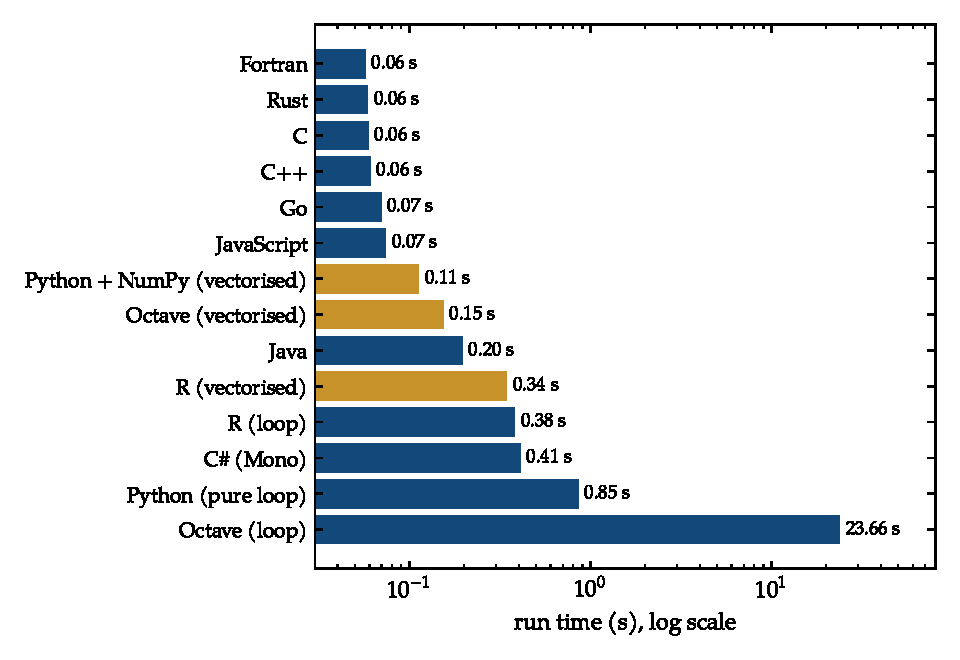
\includegraphics[width=0.85\linewidth]{figures/benchmark.pdf}
\caption{Time to evaluate the trapezoidal rule with $n = 10^7$ intervals (best of three
runs, one core of a 2.1~GHz Intel Xeon server, Linux). Blue bars: an explicit loop; gold bars: a
vectorised expression. Versions: GCC/gfortran 13.3 with \code{-O2}, OpenJDK 21, Node.js
22, Go 1.24, Rust 1.97, Mono 6.8, CPython 3.13 with NumPy 2.5, GNU Octave 8.4, R 4.3.
Note the logarithmic scale.}
\label{fig:benchmark}
\end{figure}

Several lessons can be read from the figure.
\begin{itemize}
\item \textbf{The compiled languages are all about equally fast.} C, C++, Fortran and Rust
  produce essentially the same machine code; Go is close behind. The run time is dominated
  by the $10^7$ calls to $\sin$.
\item \textbf{JIT compilation works.} JavaScript, a dynamic language, runs this loop
  within about 25\% of C, thanks to the V8 JIT compiler. Java is slower here mainly because
  its \code{Math.sin} guarantees a particular accuracy in software. The old Mono runtime is
  much slower than modern .NET would be.
\item \textbf{Interpreted loops are slow.} The pure-\py loop is about 15 times slower
  than C, and the Octave loop about 400 times slower. (MATLAB's JIT engine runs such loops
  much faster than Octave; the difference shows how much the implementation matters.)
\item \textbf{Vectorisation recovers most of the speed.} NumPy and vectorised Octave
  bring the interpreted languages to within a factor of 2--3 of C, at the cost of
  allocating arrays of $10^7$ numbers (80~MB each).
\item \textbf{R's loop is surprisingly fast} here because R compiles functions and loops
  to bytecode; its vectorised version is not faster in this case because creating the large
  arrays costs as much as the loop.
\end{itemize}
Two languages are missing or misrepresented in the figure. Julia was not installed on
the computer used for the timings, so it is not shown; a compiled Julia loop is expected to
run at about the speed of C, Fortran and Rust. And C\# was timed with the old Mono runtime,
not with current .NET, which runs such a loop much faster.

Benchmarks like this one measure one narrow thing on one computer. Real programs spend
their time in many different places, and a program that is a hundred times faster but
takes a week longer to write and test is often the worse choice. Measure before you
optimise --- and optimise the part that actually takes the time.

\section{Syntax at a glance}

Table~\ref{tab:syntax} collects the basic syntax of the main languages of these notes on
one page. Use it as a quick reference when reading unfamiliar code.

\begin{sidewaystable}
\centering
\caption{Basic syntax compared. ``Index'' is the first array index; ``Block'' is how a block
of code is delimited.}
\label{tab:syntax}
\small
\setlength{\tabcolsep}{3pt}
\resizebox{\linewidth}{!}{%
\begin{tabular}{@{}>{\bfseries}l>{\ttfamily}l>{\ttfamily}l>{\ttfamily}l>{\ttfamily}l>{\ttfamily}l@{}}
\toprule
 & \normalfont\bfseries Python & \normalfont\bfseries Fortran & \normalfont\bfseries C / C++ & \normalfont\bfseries Java / C\# & \normalfont\bfseries JavaScript\\
\midrule
Comment & \# text & ! text & // text & // text & // text\\
Variable & x = 1.0 & real(dp) :: x & double x = 1.0; & double x = 1.0; & let x = 1.0;\\
Constant & G = 9.81 & real, parameter :: & const double & final / const & const g = 9.81;\\
Power & x**2 & x**2 & pow(x, 2) & Math.pow(x, 2) & x ** 2\\
Int.\ division & 7 // 2 & 7 / 2 & 7 / 2 & 7 / 2 & Math.trunc(7/2)\\
Not equal & != & /= & != & != & !==\\
And / or & and, or & .and., .or. & \&\&, || & \&\&, || & \&\&, ||\\
Block & indentation & end ... & \{ \} & \{ \} & \{ \}\\
If & if x > 0: & if (x > 0) then & if (x > 0) \{ & if (x > 0) \{ & if (x > 0) \{\\
Loop & for i in range(n): & do i = 1, n & for (i=0; i<n; i++) & for (i=0; i<n; i++) & for (let i=0; i<n; i++)\\
Function & def f(x): & function f(x) & double f(double x) & static double f(double x) & function f(x) \{\\
Array & [1.0, 2.0] & [1.0, 2.0] & \{1.0, 2.0\} & \{1.0, 2.0\} & [1.0, 2.0]\\
Index & 0 & 1 (any) & 0 & 0 & 0\\
Length & len(a) & size(a) & (pass n) / a.size() & a.length / a.Length & a.length\\
Print & print(f"\{x:.3f\}") & print \textquotesingle{}(f0.3)\textquotesingle{}, x & printf("\%.3f", x) & printf / \$"\{x:F3\}" & x.toFixed(3)\\
\midrule
 & \normalfont\bfseries MATLAB & \normalfont\bfseries R & \normalfont\bfseries Julia & \normalfont\bfseries Wolfram & \normalfont\bfseries Rust\\
\midrule
Comment & \% text & \# text & \# text & (* text *) & // text\\
Variable & x = 1.0; & x <- 1.0 & x = 1.0 & x = 1.0 & let x = 1.0;\\
Constant & {\normalfont n/a} & {\normalfont n/a} & const g = 9.81 & {\normalfont n/a} & const G: f64 = 9.81;\\
Power & x\^{}2, x.\^{}2 & x\^{}2 & x\^{}2 & x\^{}2 & x.powi(2)\\
Int.\ division & idivide / floor & 7 \%/\% 2 & div(7, 2) & Quotient[7, 2] & 7 / 2\\
Not equal & \textasciitilde= & != & != & != & !=\\
And / or & \&\&, || & \&\&, || & \&\&, || & \&\&, || & \&\&, ||\\
Block & end & \{ \} & end & [ ] & \{ \}\\
If & if x > 0 & if (x > 0) \{ & if x > 0 & If[x > 0, ...] & if x > 0.0 \{\\
Loop & for i = 1:n & for (i in 1:n) \{ & for i in 1:n & Do[..., \{i, n\}] & for i in 0..n \{\\
Function & function y = f(x) & f <- function(x) & f(x) = ... & f[x\_] := ... & fn f(x: f64) -> f64\\
Array & [1.0 2.0] & c(1.0, 2.0) & [1.0, 2.0] & \{1.0, 2.0\} & vec![1.0, 2.0]\\
Index & 1 & 1 & 1 & 1 & 0\\
Length & numel(a) & length(a) & length(a) & Length[a] & a.len()\\
Print & fprintf(\textquotesingle{}\%.3f\textquotesingle{}, x) & sprintf("\%.3f", x) & @printf("\%.3f", x) & NumberForm[x, \{4,3\}] & println!("\{:.3\}", x)\\
\bottomrule
\end{tabular}}
\end{sidewaystable}

\begin{exercises}
\item Choose two languages from this chapter that you have not used before. Install them
  (or use an online compiler) and run their versions of the Rosetta program.
\item Add a fourth task to the \py program: solve the $3\times3$ linear system with
  \code{gauss\_solve}. Then add the same task to the C version.
\item Change the trapezoidal rule to Simpson's rule in three languages of your choice.
  Verify that the error for $n = 100$ drops to about $10^{-8}$.
\item Repeat the speed test on your own computer with \py (loop and NumPy) and one compiled
  language. Do you see the same ratios?
\item Add a Numba-compiled version of the trapezoidal loop (\code{from numba import njit})
  to the \py benchmark. How close does it come to C?
\item Find the Rosetta Code website (\url{https://rosettacode.org}) and look up a task of
  your choice, such as ``Matrix multiplication'' or ``Numerical integration''. Compare the
  solutions in three languages.
\end{exercises}
